% Start Header
\documentclass[11pt]{article}

\usepackage{amsmath}
\usepackage{amssymb}
\usepackage{fancyhdr}
\usepackage{listings}
\usepackage{color}
\usepackage{graphicx}
\graphicspath{ {images/} }
\usepackage{hyperref}
\usepackage{mathtools}

\newcommand\Myperm[2][n]{\prescript{#1\mkern-2.5mu}{}P_{#2}}
\newcommand\Mycomb[2][n]{\prescript{#1\mkern-0.5mu}{}C_{#2}}

\definecolor{dkgreen}{rgb}{0,0.6,0}
\definecolor{gray}{rgb}{0.5,0.5,0.5}
\definecolor{mauve}{rgb}{0.58,0,0.82}

\def\code#1{\texttt{#1}}

\lstset{frame=tb,
  language=Java,
  aboveskip=3mm,
  belowskip=3mm,
  showstringspaces=false,
  columns=flexible,
  basicstyle={\small\ttfamily},
  numbers=none,
  numberstyle=\tiny\color{gray},
  keywordstyle=\color{blue},
  commentstyle=\color{dkgreen},
  stringstyle=\color{mauve},
  breaklines=true,
  breakatwhitespace=true,
  tabsize=3
}

\oddsidemargin0cm
\topmargin-2cm     %I recommend adding these three lines to increase the 
\textwidth16.5cm   %amount of usable space on the page (and save trees)
\textheight23.5cm  

\newcommand{\question}[2] {\vspace{.25in} \hrule\vspace{0.5em}
\noindent{\bf #1: #2} \vspace{0.5em}
\hrule \vspace{.10in}}
\renewcommand{\part}[1] {\vspace{.10in} {\bf (#1)}}

\newcommand{\myname}{Chang-Hyun Mungai}

\setlength{\parindent}{0pt}
\setlength{\parskip}{5pt plus 1pt}
 
\pagestyle{fancyplain}
\lhead{\fancyplain{}{\textbf{\myhwnum}}}      % Note the different brackets!

% End Header

\newcommand{\myhwnum}{Pointers Notes}

\begin{document}

\medskip                        % Skip a "medium" amount of space
                                % (latex determines what medium is)
                                % Also try: \bigskip, \littleskip

\thispagestyle{plain}
\begin{center}                  % Center the following lines
{\Large Pointers}
\end{center}

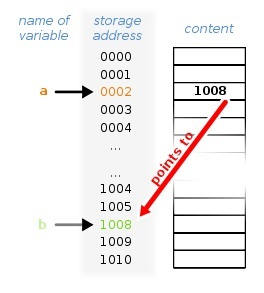
\includegraphics{pointer}

\question{Definition}

\begin{itemize}
  \item object whose value refers to another value stored elsewhere in the computer memory using its memory address
\end{itemize}

\question{Syntax}

\begin{itemize}
  \item C
  \begin{itemize}
  \item \code{int *ptr;}
    \begin{itemize}
    \item This declares ptr as the identifier pointer that points to an object of type int
    \end{itemize}
   \item
   \begin{lstlisting}
int a = 5;
	int *ptr = NULL;
	ptr = &a;
   \end{lstlisting}
    \begin{itemize}
    \item Assigns the value of the address of a to ptr
    \item example: if a is stored at memory location of 0x8130 then the value of ptr will be 0x8130 after the assignment
    \item To dereference the pointer, an asterisk is used again
    \end{itemize}
  \item \code{*ptr = 8;}
    \begin{itemize}
    \item This means take the contents of ptr (which is 0x8130), "locate" that address in memory and set its value to 8
    \end{itemize}
  \end{itemize}
\end{itemize}

\question{sources}

\begin{itemize}
\item \url{https://en.wikipedia.org/wiki/Pointer_(computer_programming)}
\end{itemize}

\end{document}

